\chapter[Ciclos de Vida para o Desenvolvimento do Projeto]{Ciclos de Vida para o Desenvolvimento do Projeto}
\label{chap:cicloDeVida}

	Modelos de ciclo de vida captam um conjunto de atividades e a maneira como elas se relacionam. Permitem ter uma visão geral do esforço de desenvolvimento, de forma que o progresso possa ser rastreado; os resultados, especificados; os recursos, alocados; as metas estabelecidas; e assim por diante.

	Nas seções a seguir serão analisadas os ciclos de vida mas utilizados nos projetos atuais.

	\section[Análise do Modelo Ciclo de Vida Simples]{Análise do Modelo de Ciclo de Vida Simples}
	\label{sec:cicloDeVida_Simples}

		Este modelo não deve ser visto como prescritivo. Ele inicia com a identificação de necessidades e requisitos. A partir disto, são elaborados alguns designs, em seguida, são desenvolvidos e avaliados.
		
		Composto por quatro atividades básicas, este modelo favorece a revisão iterativa e incentiva o design centrado no usuário.
		
		A primeira atividade proposta neste modelo é a identificação das necessidades do usuário, ou seja, quais atividades do usuário serão apoiadas pelo sistema. Em seguida, com base nas necessidades identificadas, são estabelecidos os requisitos que vão apoiar tais atividades.
		
		Logo após a identificação das necessidades e requisitos, vem o design propriamente dito, onde serão propostas algumas soluções alternativas para o que foi identificado anteriormente. Em seguida, há a prototipação destas soluções para que elas possam ser avaliadas pelos usuários. Tal avaliação tem por objetivo verificar se as soluções propostas apoiam adequadamente as atividades dos usuários. Com base nos resultados obtidos desta avaliação, é possível que os designers identifiquem novas necessidades e requisitos para o sistema sendo projetado, melhorando desta maneira a qualidade da interface do sistema através da revisão iterativa do artefato, antes que a sua versão final seja produzida.
		
		O modelo de ciclo de vida simples incorpora características fundamentais para qualquer processo de projeto da interação.

		\begin{figure}[h]
			\centering
			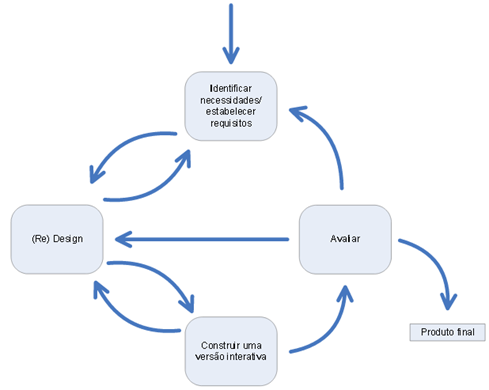
\includegraphics[scale=0.6]{ciclo_De_Vida_Simplesciclo_De_Vida_Simples}
			\caption[Modelo Ciclo de Vida Simples]{Modelo Ciclo de Vida Simples. \cite{designEInteracao}}
			\label{fig:ciclo_De_Vida_Simplesciclo_De_Vida_Simples}
		\end{figure}

	\newpage
	
	\section[Análise do Modelo Ciclo de Vida de Engenharia de Usabilidade]{Análise do Modelo Ciclo de Vida de Engenharia de Usabilidade}
	\label{sec:cicloDeVida_EU}
		A usabilidade é desenvolvida através de um conjunto de atividades, que dependendo do paradigma para o ciclo de vida do produto, podem estar encadeadas de diversas formas: em cascata, em ciclos de prototipagem e testes, em espirais evolucionárias ou em diagonais de reutilização. \cite{designEInteracao}

		A pertinência de um modelo ou outro vai depender do contexto do desenvolvimento, em particular, do caráter inovador das propostas, do conhecimento do domínio do sistema, dos recursos e do tempo disponível, da experiência de equipe, etc. Mas seja qual for o modelo escolhido, as atividades necessárias para o desenvolvimento pertencerão a uma das três categorias ou perspectivas principais: Análise, Síntese e Avaliação.

		A perspectiva da análise se refere ao esforço para estabelecer uma compreensão do contexto de operação do sistema, a partir da sua subdivisão em aspectos ligados aos usuários, a seus objetivos e ao ambiente de trabalho. Para o desenvolvimento da usabilidade, a análise não só de uma situação existente, mas também de uma futura, é importante, uma vez que é por meio destas atividades que se estabelece um foco e um processo de comunicação e de envolvimento do usuário no desenvolvimento. Quanto mais frequente e progressivo o processo de análise, maior será a qualidade nas decisões de projeto.

		Perspectiva da Síntese - O processo de síntese de uma interface com o usuário deve ser fruto de uma sequência lógica de etapas. Mesmo um protótipo, a partir do qual a interface evolui, não aparece do nada, como pretendem os métodos populares de engenharia de software. A lógica da perspectiva de síntese (especificação, projeto e implementação) de uma nova interface com o usuário, apresenta a seguinte estrutura de atividades:

		\begin{itemize}
			\item{A usabilidade a alcançar, quantitativa e qualitativamente;}
			\item{O novo contexto de operação, incluindo a nova estrutura do trabalho;}
			\item{O estilo para a interface (guias de estilo);}
			\item{A estrutura e o processo da nova interface.}
		\end{itemize}

		Perspectiva da Avaliação - O entendimento da avaliação como perspectiva é fundamental para o sucesso no desenvolvimento de interfaces com o usuário. Todas as metas (resultados intermediários) deste processo devem ser verificadas (por seus projetistas) e validadas (por seus usuários). Em particular, os testes da usabilidade devem ter como eixos de exame:

		\begin{itemize}
			\item{a eficácia da interação humano-computador face a efetiva realização das tarefas por parte dos usuários;}
			\item{a eficiência desta interação, face os recursos empregados (tempo, quantidade de incidentes, passos desnecessários, busca de ajuda, etc.);}
			\item{a satisfação ou insatisfação (efeito subjetivo) que ela possa trazer ao usuário.}
		\end{itemize}

		Estes objetivos devem ser pensados em relação aos diferentes contextos de operação previstos para o sistema.
		
		A usabilidade de um sistema está sempre associada às características de determinados tipos de usuários, tarefas, equipamentos e ambientes físicos e organizacionais. Assim, um problema de usabilidade pode se fazer sentir fortemente em determinados contextos de operação e ser menor ou mesmo imperceptível, em outros.

		A imagem a seguir ilustra o ciclo de vida da Engenharia de Usabilidade.

		\begin{figure}[h]
			\centering
			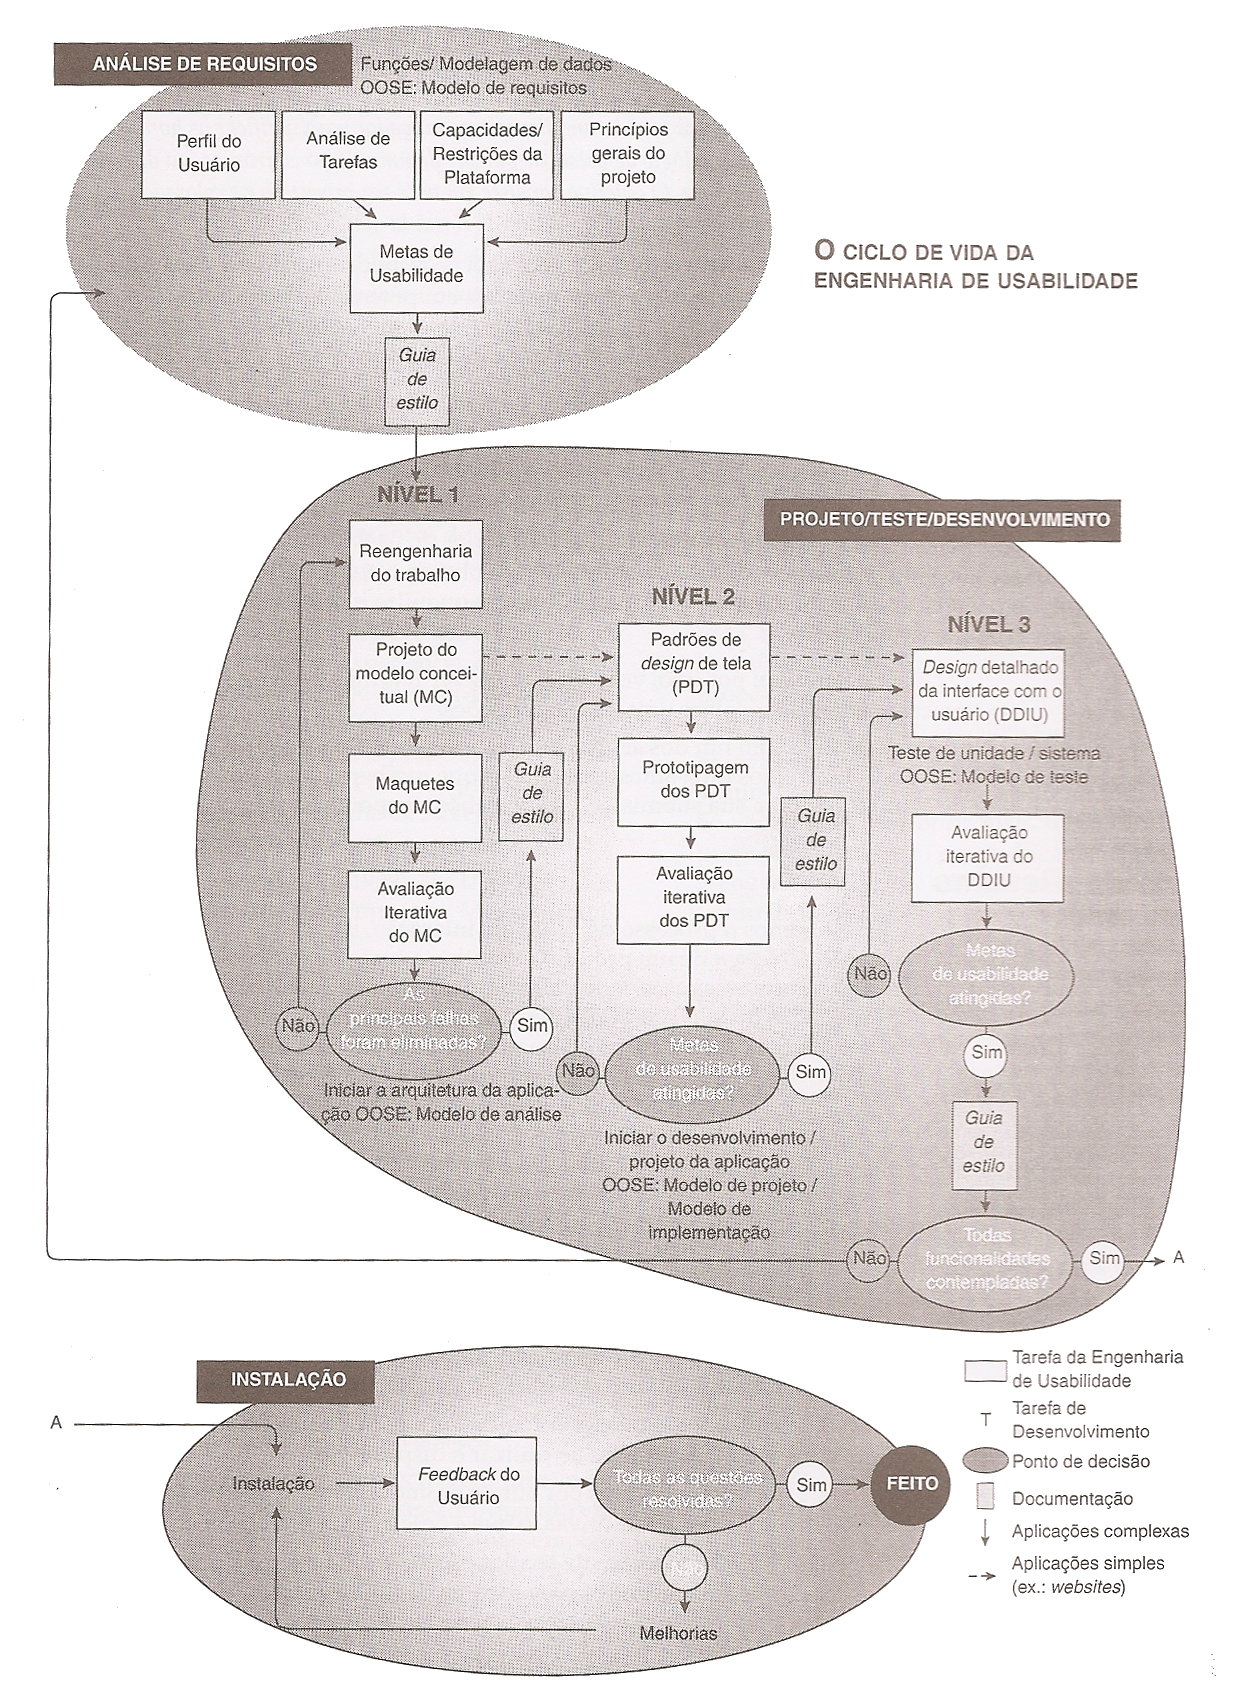
\includegraphics[scale=0.35]{cicloUE}
			\caption[Modelo do Ciclo Engenharia de Usabilidade]{Modelo do Ciclo Engenharia de Usabilidade. \cite{designEInteracao}}
			\label{fig:cicloUE}
		\end{figure}